\documentclass[10pt]{article}
\usepackage[polish]{babel}
\usepackage[utf8]{inputenc}
\usepackage[T1]{fontenc}
\usepackage{amsmath}
\usepackage{amsfonts}
\usepackage{amssymb}
\usepackage[version=4]{mhchem}
\usepackage{stmaryrd}
\usepackage{graphicx}
\usepackage[export]{adjustbox}
\graphicspath{ {./images/} }

\title{EGZAMIN WSTĘPNY Z MATEMATYKI }

\author{}
\date{}


\begin{document}
\maketitle
Zestaw składa się z 30 zadań. Zadania 1-10 oceniane będą w skali 0-2 punkty, zadania \(11-30\) w skali \(0-4\) punkty. Czas trwania egzaminu - 240 minut.

Powodzenia!

\begin{enumerate}
  \item Rozwiązać nierówność \(x-\frac{2}{x} \geqslant 1\).
  \item Dla jakich \(a\) równanie \(x^{2}+a x+a-1=0\) posiada co najmniej jeden pierwiastek rzeczywisty?
  \item Rozwiązać równanie \(\sqrt{x}+2=x\).
  \item Trzy liczby tworzą ciąg arytmetyczny o sumie równej 18. Największa z nich jest równa 9 . Wyznaczyć pozostałe liczby.
  \item Rozwiązać nierówność \(\left(\frac{1}{2}\right)^{|x-3|} \geqslant \frac{1}{4}\).
  \item Dany jest sześcian o krawędzi a Obliczyć objętość kuli stycznej do wszystkich krawędzi tego sześcianu.
  \item Obliczyć \((\sqrt[3]{4})^{\frac{3}{2^{2 \log _{3} 2}}}\).
  \item Dla jakich \(x \in(0 ; \pi)\) spełniona jest nierówność \(\operatorname{ctg}^{2} x \geqslant 3\) ?
  \item Obliczyć granicę \(\lim _{n \rightarrow \infty} \frac{(n+2)!}{n^{2} \cdot n!}\).
  \item Graficznie rozwiązać nierówność \(\log _{\frac{1}{2}}|x| \geqslant x^{2}-1\).
  \item Wielomian \(w(x)=x^{3}-3 x+a\) rozłożyć na czynniki wiedząc, że liczba -1 jest jego pierwiastkiem.
  \item Dla jakich parametrów \(m\) układ równań \(\left\{\begin{array}{r}m x-2 y=1 \\ 8 x-m y=2\end{array}\right.\) jest sprzeczny?
  \item Trójkąt ma boki długości 6,8 i 10. Obliczyć promień okręgu opisanego na tym trójkącie i promień okręgu wpisanego w ten trójkąt.
  \item Napisać równanie stycznej do wykresu funkcji \(f(x)=4 \sqrt[3]{8+\sin 3 x}\) w punkcie \(x_{0}=0\).
  \item Dla jakich wartości parametru \(m\) okręgi \(x^{2}+y^{2}-2 x=0\) oraz \(x^{2}+(y-m)^{2}=9\) są styczne wewnętrznie?
  \item Wyznaczyć dziedzinę funkcji \(f(x)=\sqrt{\log \left(3^{x}-2^{x}+1\right)}\).
  \item Trzy razy rzucamy dwiema kostkami do gry. Jakie jest prawdopodobieństwo tego, że co najmniej raz suma oczek będzie większa od 9 ?
  \item Obliczyć granicę \(\lim _{x \rightarrow 0} \log _{2}\left(\frac{x^{2}}{1-\cos 4 x}\right)\).
  \item Niech \(f(m)\) oznacza liczbę pierwiastków równania \(\left|4 x^{2}-4 x-3\right|=m\). Narysować wykres funkcji \(f(m)\).
  \item Na prostej \(y-x-1=0\) znaleźć punkt \(A\) taki, że pole trójkąta o wierzchołkach w punktach \(A, B(4,-1)\) i \(C(4,3)\) jest równe 2.
  \item Obliczyć kat między wektorami \(\vec{a} \mathrm{i} \vec{b}\), jeśli wiadomo, że wektory \(\vec{u}=-\vec{a}+4 \vec{b}\) \(\mathrm{i} \vec{v}=3 \vec{a}+2 \vec{b}\) są prostopadłe i \(|\vec{a}|=|\vec{b}|=1\).
  \item Uzasadnić, że prosta \(4 x+2 y-3=0\) jest równoległa do prostej \(\left\{\begin{array}{l}x=-t+1 \\ y=2 t-3\end{array}\right.\). Obliczyć odległość między tymi prostymi.
  \item Zbadać monotoniczność funkcji \(f(x)=x^{3}-3 x^{2}+4 x+\cos x\).
  \item W trapez równoramienny o polu \(S\) wpisano czworokąt tak, że jego wierzchołki są środkami boków trapezu. Jaki to czworokąt? Obliczyć jego pole.
  \item Niech \(A\) i \(B\) będą zdarzeniami losowymi takimi, że \(P(A)=0,7\) i \(P(B)=0,9\). Wykazać, że \(P(A \mid B) \geqslant \frac{2}{3}\).
  \item Obliczyć granice \(\lim _{x \rightarrow+\infty}\left(x-\sqrt{x^{2}-x+1}\right)\) oraz \(\lim _{x \rightarrow-\infty}\left(x-\sqrt{x^{2}-x+1}\right)\).
  \item Rozwiązać równanie \(1+\frac{1}{2 \sin x}+\frac{1}{4 \sin ^{2} x}+\cdots=\frac{2}{\sin x}\).
  \item Wyznaczyć największą i najmniejszą wartość funkcji \(f(x)=\frac{1}{\sin x+\cos x} \quad \mathrm{w}\) przedziale \(\left\langle 0 ; \frac{\pi}{2}\right\rangle\).
  \item Podać definicję ciągu ograniczonego. Następnie wykazać, że ciąg
\end{enumerate}

\[
a_{n}=\frac{1}{n+1}+\frac{1}{n+2}+\cdots+\frac{1}{2 n}
\]

jest ograniczony.\\
30. Podać i udowodnić warunek konieczny istnienia maksimum lokalnego funkcji różniczkowalnej.

\section*{Odpowiedzi do kolejnych zadań:}
\begin{enumerate}
  \item \(x \in\langle-1 ; 0) \cup\langle 2 ;+\infty)\);
  \item dla każdej liczby \(a \in R\);
  \item \(x=4\);
  \item liczbami tymi są \(a_{1}=3, a_{2}=6\) i \(a_{3}=9\);
  \item \(x \in\langle 1 ; 5\rangle\);
  \item \(V=\frac{1}{3} \pi a^{3} \sqrt{2}\);
  \item \((\sqrt[3]{4})^{\frac{3}{2 \log _{3} 2}}=3\);
  \item \(x \in\left(0 ; \frac{\pi}{6}\right\rangle \cup\left\langle\frac{5}{6} \pi ; \pi\right)\);
  \item 1 ;
  \item \(x \in\langle-1 ; 0) \cup(0 ; 1\rangle\);
  \item \(w(x)=(x+1)^{2}(x-2)\);
  \item \(m=-4\);
  \item \(R=5\) i \(r=2\);
  \item \(y=x+8\);
  \item \(m= \pm \sqrt{3}\);
  \item \(x \geqslant 0\);
  \item \(P=\frac{91}{216}\);
  \item -3 ;
  \item 
\end{enumerate}

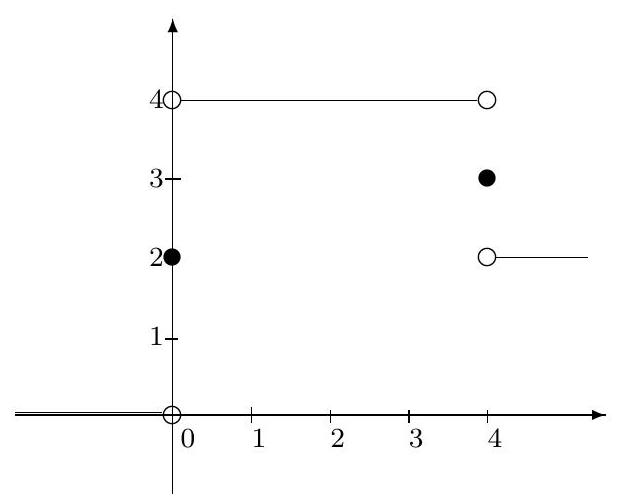
\includegraphics[max width=\textwidth, center]{2024_11_21_7d1c5282a8fcc5ab838ag-3}\\
20. \(A(3,4)\) lub \(A(5,6)\);\\
21. \(\frac{2}{3} \pi\);\\
22. \(d=\frac{\sqrt{5}}{2}\);\\
23. Zauważmy, że spełniona jest nierówność \(3 x^{2}-6 x+4 \geqslant 1\) (i nawet \(3 x^{2}-6 x+4>1\), gdy \(x \neq 1\) ). Stąd już wynika, że pochodna funkcji \(f(x)\) jest dodatnia,

\[
f^{\prime}(x)=3 x^{2}-6 x+4-\sin x>0 \quad \text { (także dla } x=1 \text { ), }
\]

i dlatego fnkcja \(f(x)\) jest rosnąca;\\
24. czworokąt jest rombem o polu \(P=S / 2\);\\
25. \(P(A \mid B)=\frac{P(A \cap B)}{P(B)}=\frac{P(A)+P(B)-P(A \cup B)}{P(B)} \geqslant \frac{0,7+0,9-1}{0,9}=\frac{2}{3}\);\\
26. \(1 / 2 \mathrm{i}-\infty\);\\
27. \(x=\frac{\pi}{2}+2 k \pi\) i \(k\) jest liczbą całkowita;\\
28. \(M=1\) i \(m=\frac{\sqrt{2}}{2}\);\\
29. \(\left(a_{n}\right)\) jest ograniczony, gdy istnieje liczba rzeczywista \(M\) taka, że \(\left|a_{n}\right| \leqslant M\) dla każdej liczby naturalnej \(n\). Dla rozważanego ciągu i dla każdej liczby naturalnej \(n\) jest

\[
\left|a_{n}\right|=a_{n}=\frac{1}{n+1}+\frac{1}{n+2}+\cdots+\frac{1}{2 n} \leqslant \frac{1}{n+1}+\frac{1}{n+1}+\cdots+\frac{1}{n+1}=\frac{n}{n+1} \leqslant 1,
\]

więc ciąg ten jest ograniczony.\\
30. Jeśli funkcja \(f(x)\) jest różniczkowalna w punkcie \(x_{0}\) i jeśli ma ona maksimum lokalne w tym punkcie, to \(f^{\prime}\left(x_{0}\right)=0\).


\end{document}